
\section{SECDA-DSE}
\label{method}

% SECDA-DSE extends the SECDA ecosystem, which comprise of various tools and components present in SECDA including simulation profiler, AXI APIs, and scheduler by introducing an automated framework for exploring hardware accelerator design spaces.
SECDA-DSE extends the SECDA ecosystem, which comprise of various tools and components present in SECDA including AXI APIs, hardware monitors and simulation profiler by introducing an automated framework for exploring hardware accelerator design spaces.
Figure~\ref{fig:SECDA-DSE Overview} shows the overall architecture of SECDA-DSE, which consists of two main components: (i) \textbf{DSE Explorer}\textbf{:} Responsible for generating and evaluating hardware configurations; (ii)  \textbf{LLM Stack}\textbf{:} Responsible for reasoning over the design space and guiding exploration strategies.

The framework takes as inputs: A target AI workload (e.g., CNNs, LLMs); A target FPGA device (e.g., PYNQ-Z1, Kria KV260); Architectural directives for exploration (e.g., tiling strategies, compute unit dimensions, memory hierarchy parameters). 
Based on these inputs, SECDA-DSE generates candidate accelerator architectures and evaluates them using the SECDA ecosystem.
The evaluation results are then further used to refine subsequent design iterations through a human-in-the-loop feedback for reinforcement. 


\begin{figure}[!tb]
  \centering
  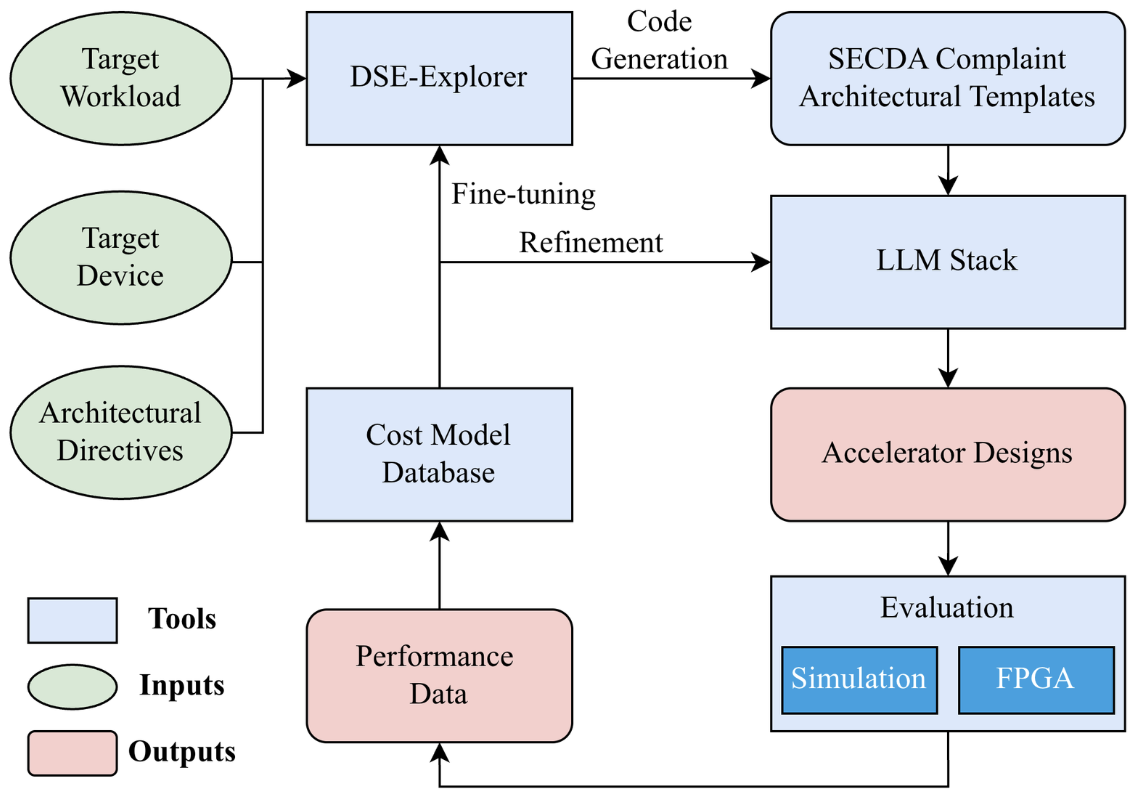
\includegraphics[width=0.89\linewidth]{img/SECDA-DSE-Overview.png}
  \caption{SECDA-DSE framework architecture showing the interaction between the DSE Explorer and the LLM Stack.}
  \label{fig:SECDA-DSE Overview}
  \Description{SECDA-DSE framework architecture showing the interaction between the DSE Explorer and the LLM Stack.}
\end{figure}


More specifically, the workflow begins with user inputs that are provided to the DSE Explorer, which generates hardware configurations and produces SECDA-native architecture that follows SECDA defined architectural guidelines and patterns.
The templates are then processed by the LLM Stack, which performs reasoning-driven refinement of the design space and generates the final accelerator designs.

The resulting designs are evaluated through simulation using the SECDA-TFLite toolkit~\cite{haris2023secda}, producing performance metrics such as execution latency, resource utilization, and data movement costs. These metrics are collected as performance data and stored in a cost model database, which is then used to guide subsequent exploration iterations through refinement and fine-tuning. By incorporating this feedback-driven loop, SECDA-DSE enables iterative improvement of accelerator configurations.

To support this iterative exploration process, SECDA-DSE is designed as a modular orchestration framework in which each component exposes an API endpoint for data interchange. The DSE Explorer generates candidate architectural parameter sets (e.g., tiling factors, compute array dimensions, memory allocation parameters) and instantiates them into SECDA-compliant accelerator templates. These templates are then passed to the LLM Stack, which retrieves relevant SECDA-TFLite implementation context, reasons over prior hardware datapoints, and proposes refined candidate configurations. Each generated design is evaluated through SECDA-based simulation and, where required, downstream synthesis and hardware execution flows, with the resulting performance and resource metrics stored in the cost model database for reuse in subsequent iterations.


The DSE Explorer and the LLM Stack interact iteratively rather than sequentially. The DSE Explorer proposes candidate parameter permutations and produces summarized hardware data-points, while the LLM Stack consumes these data-points together with retrieved implementation context to rank, refine, or reject candidate designs before the next exploration round. This interaction enables SECDA-DSE to combine structured parameter exploration with reasoning-guided design refinement while also harnessing a Chain-of-Thought (CoT) prompting approach which enforces the LLM to take instructions and step by step.


%*************************************************************************************************

\subsection{DSE Explorer}

The DSE Explorer performs the automated exploration of the accelerator design space.
It is responsible for generating and evaluating candidate accelerator configurations within the SECDA-DSE framework. As shown in Figure~\ref{fig:DSE-Explorer}, its primary objective is to navigate the large hardware design space associated with FPGA-based AI accelerators by combining structured exploration with feedback from evaluation results.

The DSE explorer operates based on three primary inputs: the target AI workload, the target FPGA device, and a set of architectural directives that constrain or guide the exploration process.
Using this information, it generates accelerator configurations that conform to SECDA-native architectural templates, enabling integration with the existing SECDA design ecosystem. 
The DSE Explorer works by taking in an accelerator design (generated by the LLM Stack or initially by an expert designer) with pre-defined hardware parameters and exploring the permutations suggested by the LLM Stack.
Each permutation generates a design run folder that includes the source code, HLS-generated RTL code, and the FPGA-mapped design.
The FPGA-mapped design is the evaluated design, and performance metrics are collected. 
Alongside this, the resource utilization of the accelerator design is used to generate a summarized set of "results" for each of the permutation run.
The summarized results along with the source code for the run are later fed into the LLM Stack as part of the "hardware data points".


\begin{figure}[!tb]
  \centering
  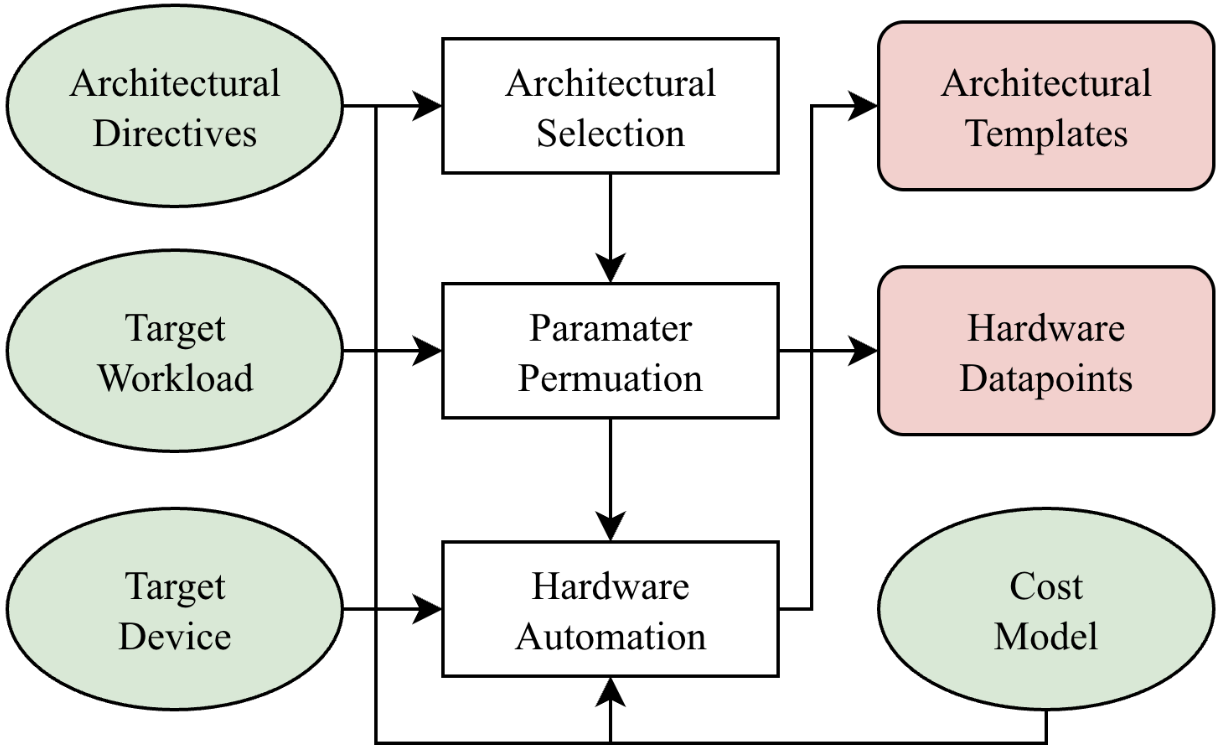
\includegraphics[width=0.8\linewidth]{img/DSE-Explorer.png}
  \caption{Workflow of the DSE Explorer.}
  \label{fig:DSE-Explorer}
  \Description{Workflow of the DSE Explorer.}
\end{figure}


%*************************************************************************************************

\subsection{LLM Stack}

The LLM Stack acts as an intelligent reasoning and orchestration layer within SECDA-DSE, guiding the exploration of the hardware design space generated by the DSE Explorer. Its primary objective is to analyze accelerator configurations, reason about architectural trade-offs, and refine exploration strategies based on evaluation feedback and historical performance data logs.

Figure~\ref{fig:LLM STACK} provides a block representation of its various modules and their interactions within and across the stack. The LLM Stack consists of two major modules: the Retrieval Augmented Generation Module (RAG) and the Evaluation module with external Model Context Protocol (MCP)-based API calls to access SECDA components. 


\begin{figure}[!tb]
  \centering
  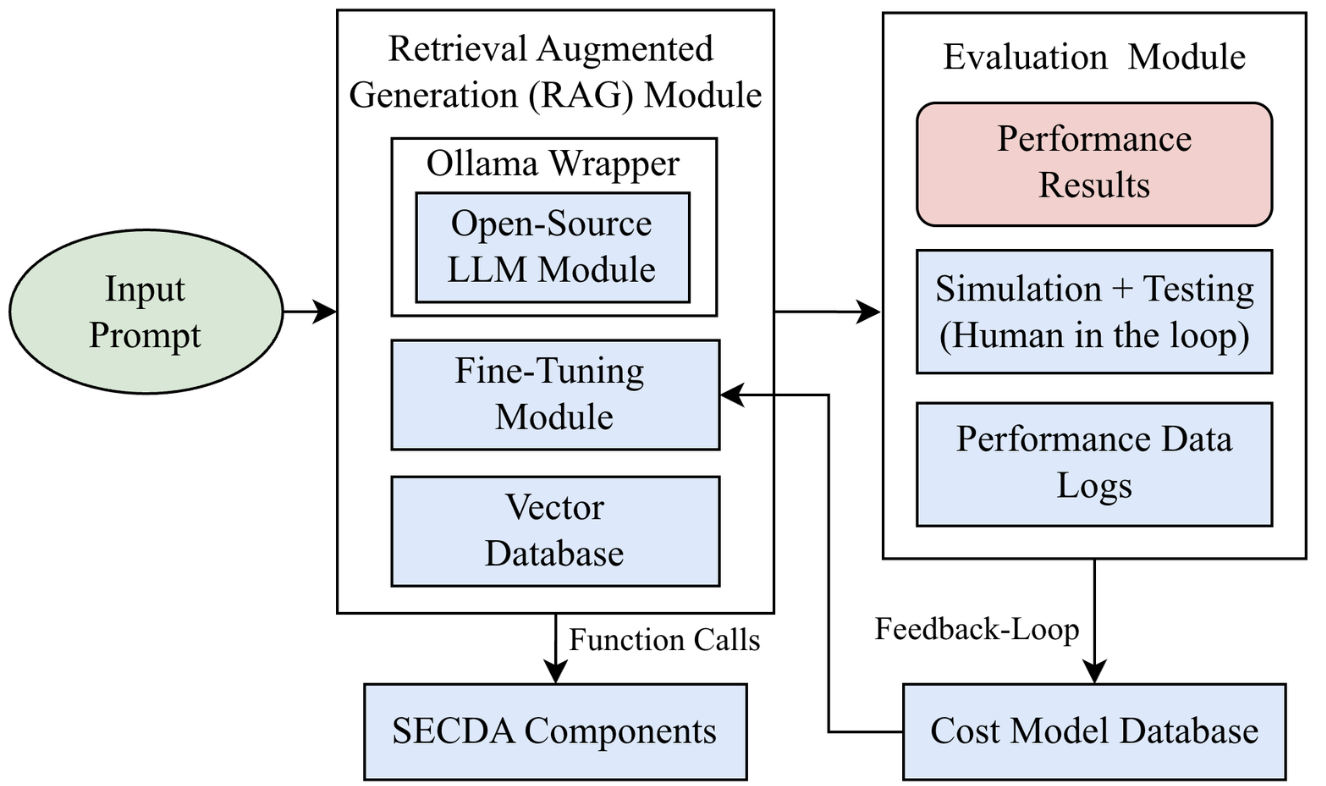
\includegraphics[width=0.99\linewidth]{img/LLM_STACK.png}
  \caption{LLM Stack Architecture illustrating various components and interactions.}
  \label{fig:LLM STACK}
  \Description{LLM Stack Architecture}
\end{figure}


\subsubsection{Retrieval Augmented Generation Module (RAG)}

The full LLM Stack pipeline is developed in a modular way using the open-source framework Ollama~\cite{ollama} for inference on-device. Ollama also enables switching between newer LLMs with ease without requiring any additional code changes for integration, making the tool easy to use for the end-user.

RAG allows the LLM to retrieve relevant information and have enough context of SECDA through a vectorized database consisting of the SECDA-TFLite code-base~\cite{haris2023secda} indexed for search through added comments. 
The RAG module does not expose the full SECDA-TFLite codebase or complete raw hardware logs at each iteration. Instead, it retrieves only the most relevant code fragments, template definitions, and API-level context required for the current design decision. This approach allows to maintain token limit while providing enough context to the LLM for making informed decisions.

Note that the LLM Stack also incorporates a parameter-efficient fine-tuning module, which adapts the LLM using data generated during the exploration process. Performance metrics obtained from simulation and FPGA execution are collected as the hardware data points and stored within the cost model database. 
In this setting, the fine-tuning dataset is constructed from previously explored accelerator designs and their associated evaluation outcomes. Each training data point includes the proposed architectural configuration, workload and device context, and the resulting feedback signals including simulation success, latency, and resource utilization. These signals enable supervision for adapting the model toward generating configurations that are both performance centric and feasible.

In addition to retrieval-based grounding, the LLM Stack employs CoT prompting as shown in Figure~\ref{fig:COT}. CoT enables structured and multi-step reasoning when exploring architectures and guides the LLM to generate intermediate reasoning steps before producing final outputs. This aims to improve its ability to analyze complex design constraints and architectural trade-offs without the extensive need for a bigger model with a pre-enabled thinking node available.


\begin{figure}[!tb]
  \centering
  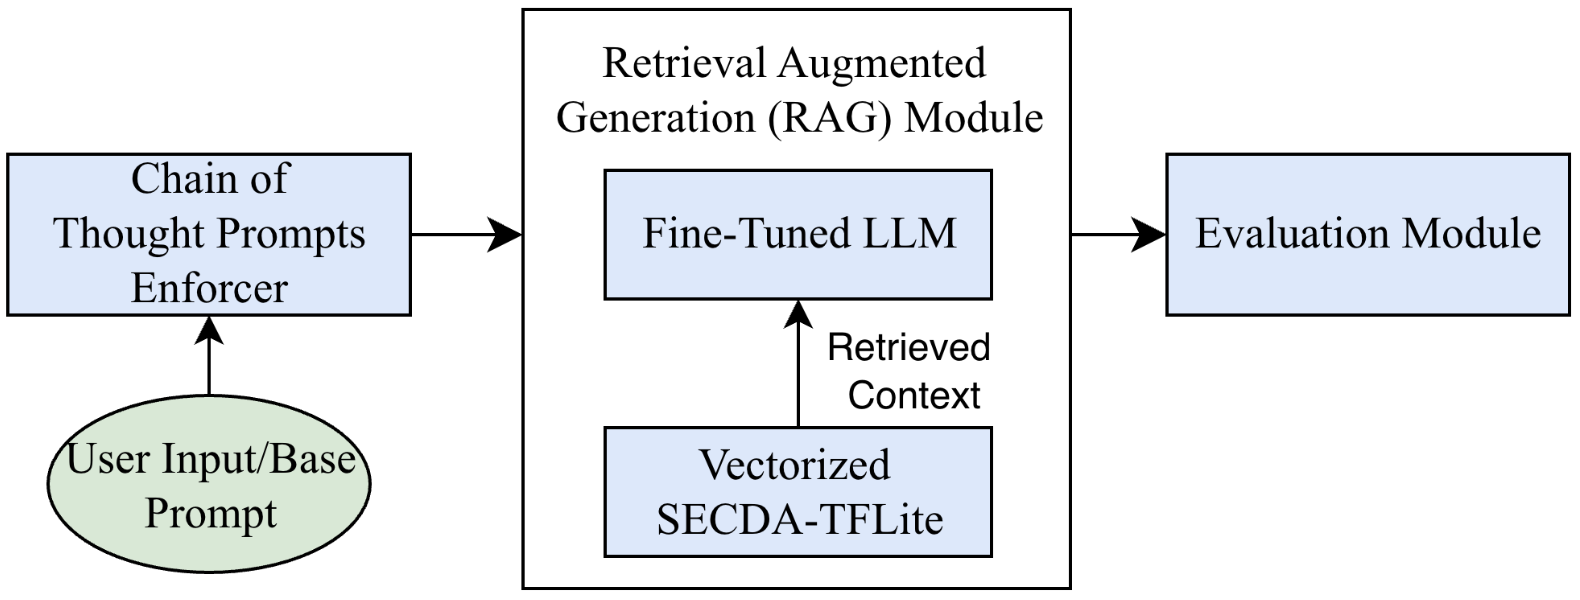
\includegraphics[width=0.98\linewidth]{img/COT.png}
  \caption{Block diagram showing how Chain-of-Thought (CoT) component is used for improving prompt structure.}
  \label{fig:COT}
  \Description{Block diagram showing how Chain-of-Thought (CoT) component is used for improving prompt structure}
\end{figure}


\subsubsection{Evaluation module}

The Evaluation module is responsible for assessing the performance and feasibility of the generated accelerator designs. Its primary role is to provide feedback that guides the iterative DSE process, as shown in Figure~\ref{fig:LLM STACK}. The module evaluates each accelerator configuration through a combination of simulation-based analysis and hardware execution initially having a human-in-the-loop but aimed to further automate and take the human-out-of-the-loop once the data-log size grows, enabling quick validation of design decisions.

The evaluation workflow begins with SystemC-based simulation, which allows the accelerator architecture to be tested within a high-level simulation environment. SystemC simulation enables rapid verification of functional correctness and provides early estimates of performance metrics such as execution latency, hardware resource estimation, and the data movement costs. These results from executions are then saved in the database, which are further passed for fine-tuning the base LLM.

To reduce invalid design proposals, SECDA-DSE constrains design generation through SECDA-compliant architectural templates and device-aware parameter ranges rather than allowing unconstrained free-form design generation. 
Candidate accelerator configurations are therefore bounded by workload requirements, and architectural directives before evaluation. Further, as shown in ~\ref{fig:LLM STACK}, there is a human-in-the-loop for testing the generated design. Any infeasible or invalid configurations that fail simulation, violate hardware resource limits, or cannot progress through downstream tool flows are rejected and logged as negative hardware data points for future refinement.

Note that the LLM Stack uses Low-Rank Adaptation (LoRA) as a parameter-efficient fine-tuning mechanism. LoRA~\cite{hu2022lora} is a widely used technique for adapting LLMs without updating the full set of model parameters. 
Instead of retraining the entire model, LoRA freezes the original pretrained weights and introduces small trainable low-rank matrices into the selected layers of the LLM architecture, enabling task-specific adaptation with fewer trainable parameters.

% To reduce the risk of converging prematurely to locally optimal designs, SECDA-DSE preserves exploration diversity across iterations rather than only exploiting the current best-performing configuration by evaluating multiple candidate parameter permutations and fine-tuning both successful and unsuccessful hardware data points, and allowing the LLM Stack to reason over broader design trade-offs.

To reduce the risk of premature convergence to locally optimal designs, SECDA-DSE maintains exploration diversity across iterations instead of focusing only on the current best-performing configuration. It does so by evaluating multiple candidate parameter permutations, refining the search based on both successful and unsuccessful hardware data points, and enabling the LLM Stack to reason over a broader range of design trade-offs before generating new accelerator designs for the target AI workload.
